\documentclass[conference]{IEEEtran}

\usepackage{mathptmx} % Times Roman Font

\usepackage{helvet} % Arial/Helvetica font
\renewcommand{\familydefault}{\sfdefault} % Makes serif text all Helvetica

\usepackage[left=0.5cm, right=0.5cm, top=0.5cm]{geometry} % Sets the page margins

\usepackage{graphicx}

\usepackage{multicol}
\usepackage{float}

\usepackage{caption}

\captionsetup[table]{skip=10pt} % Adjusts space between table and caption

\usepackage{ragged2e}

\usepackage{array}
\newcolumntype{L}[1]{>{\raggedright\arraybackslash}p{#1}}

\title{Case Study 2: Clinical Trial}
\date{}

\begin{document}
\justifying

\maketitle

\section{Introduction} 
This document outlines a draft protocol for a clinical trial studying the efficacy of preoperative rehabilitation and early mobilisation for upper limb arthroplasty (Shoulder replacements).

Prehabilitation before surgery may improve recovery. It typically includes pre and post-operation exercises, lifestyle advice, and support for functional independence. These interventions may enhance clinical outcomes and quality of life, while reducing complications and prolonged rehabilitation. 

Early shoulder mobilisation post-operation may enable faster rehabilitation and functional recovery. This benefits both patients and the NHS by shortening hospital stays and lowering readmission rates.

\vspace{4pt}
This clinical study aims to answer two questions:
\begin{itemize}
    \item What is the clinical and cost-effectiveness of preoperative rehabilitation for upper limb surgery?
    \item What is the clinical and cost-effectiveness of early versus delayed shoulder mobilisation post-surgery?
\end{itemize}

\section{Methods}

Two pilot studies will be followed by a randomised control trial (RCT) if the study is determined to be feasible.

\subsection{Pilot Studies}
The pilot studies will each assess the feasibility of the two factors (prehabilitation and early mobilisation) and give insight into recruitment numbers before a larger scale RCT can be run. They will run independently with a reduced sample size and timescale to allow each hypothesis's feasibility to be assessed without influence from confounding variables and to reduce resources required.

Pilot group A will assess the feasibility of running a trial investigating the effectiveness of prehabilitation for shoulder replacements. The sample population will be randomised and divided into two equal groups. The intervention group will begin exercises and lifestyle changes 4 weeks prior to arthroplasty surgery. The control group will not receive preoperative rehabilitation.

Pilot group B will assess the feasibility of running a trial investigating the effectiveness of early shoulder mobilisation for shoulder replacements. The sample population will be randomised and divided into two groups. Both the intervention and control group will wear an adduction sling to immobilise the shoulder during the first 4 weeks post-operative. The control group will wear an adduction sling for a further 2 weeks to continue to prevent mobilisation of the shoulder.

For both pilot studies, after three months post-operation, the Shoulder Pain and Disability Index (SPADI) will be measured and compared to baseline measurements. An RCT can be carried out if either pilot study confirm feasibility of an RCT.

\subsection{Randomised Control Trial}

In order to answer both questions efficiently in a single clinical trial, an RCT with factorial design will assess the two factors with two levels implemented. A factorial design allows two trials to be run simultaneously while only requiring the patients needed for a single trial. The sample population will be randomised and divided into four groups to remove selection bias and minimise confounding variables, illustrated in Figure.~\ref{fig:RCTGroups}. Group four is the control group, receiving no treatments. The other three intervention groups will receive a combination of the two treatments.

If only one of the hypotheses is feasible, a factorial design is not required. An RCT can be run with two randomised groups - One intervention and one control group.

\begin{figure}[h]
\centering
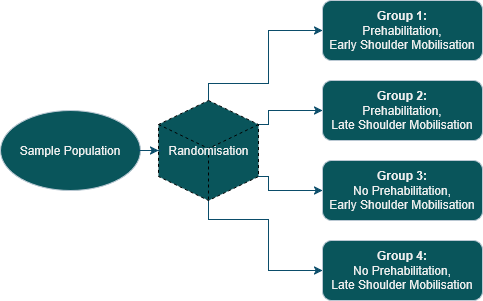
\includegraphics[width=10cm]{images/Clinical trial groups.drawio.png}
\caption{Illustration of the factorial RCT design. The sample population is randomised and divided into four equal groups.}
\label{fig:RCTGroups}
\end{figure}

To assess effectiveness of prehabilitation, exercises and lifestyle changes will begin two months prior to the arthroplasty surgery for two of the groups. The other two groups will not have any prehabilitation.

To assess effectiveness of early mobilisation of the shoulder, both the intervention and control group will wear an adduction sling to immobilise the shoulder during the first 4 weeks post-operative. The control group will wear an adduction sling for a further 2 weeks to continue to prevent mobilisation of the shoulder.

12 months post-operation, The SPADI, The American Shoulder and Elbow Surgeons (ASES) score, The Constant-Murley Score (CS), and The Oxford Shoulder Score (OSS) will be compared to baseline measurements to assess the efficacy of the treatments. For strength testing involved in the CS, the patient holds the arm in 90° abduction with the elbow extended and palm pronated. The force is measured over three trials using a spring balance on the forearm. The average is recorded only if the movement is pain-free and the position can be held. A higher score means better shoulder function and less pain.
\section{Sample Population}

Both genders may be admitted to the trials as shoulder mechanics does not differ significantly between them. Also, all ages above eighteen may be considered due to many of the proposed pain and mobility tools taking age into account when computing results. A detailed inclusion/exclusion criteria can be seen in Table.~\ref{tab:inclusion} and Table.~\ref{tab:exclusion}. Table.~\ref{tab:stopgocriteria} lists the stop/go criteria for the trials.

\subsection{Pilot Studies}

The pilot studies must have enough participants to estimate recruitment, adherence/attendance, and variability if a larger RCT were to be conducted. Each group should have approximately 15-30 participants. Therefore, 120 participants would be needed to assess both hypotheses. To increase the efficiency of the pilot studies, it may be advisable to implement a factorial design to reduce the number of participants required to assess feasibility.

\subsection{Factorial Design Randomised Control Trial}

The RCT will require more participants to accurately measure the efficacy of the treatments.  When using a factorial design, each group should have approximately 75 participants minimum, with 300 participants overall. This means that at least 150 people will receive each treatment.

\begin{table}[h!]
\centering
\caption{Inclusion Criteria}
\begin{tabular}{|p{8cm}|}
\hline
\textbf{Inclusion Criteria} \\
\hline
Adult men and women over the age of 18 \\
\hline
At least 8 weeks away from scheduled shoulder arthroplasty \\
\hline
Willing and able to attend prehabilitation sessions \\
\hline
Baseline functional limitations and pain measured \\
\hline
Patients capable of giving informed consent\\
\hline
\end{tabular}
\label{tab:inclusion}
\end{table}

\begin{table}[h!]
\centering
\caption{Exclusion Criteria}
\begin{tabular}{|p{8cm}|}
\hline
\textbf{Exclusion Criteria} \\
\hline
Previous shoulder replacement surgery \\
\hline
Planned or recent shoulder surgery other than arthroplasty \\
\hline
Inability to participate in prehabilitation exercises \\
\hline
Inability to provide informed consent\\
\hline
Other suspected shoulder pathology\\
\hline
Pregnancy\\
\hline
\end{tabular}
\label{tab:exclusion}
\end{table}

\begin{table}[!ht]
\centering
\caption{Stop/Go criteria for clinical trial on efficacy of shoulder replacement prehabilitation and early mobilisation of shoulder post upper limb arthroplasty}
% \resizebox{\textwidth}{!}{%
\begin{tabular}{|L{2cm}|L{2cm}|L{2cm}|L{2cm}|}
\hline
\textbf{Domain} & \textbf{Go} & \textbf{Review} & \textbf{Stop} \\
\hline
Recruitment & $\geq 70\%$ of eligible patients enrolled & 50–69\% enrolled & $<50\%$ enrolled \\
\hline
Retention & $\geq 80\%$ complete prehabilitation exercises and begin early mobilisation & 60–79\% retained & $<60\%$ retained \\
\hline
Prehabilitation Attendance & $\geq 75\%$ attend $\geq 75\%$ of sessions & 50–74\% attendance & $<50\%$ attendance \\
\hline
Safety & No injuries & 1–2 injuries & $\geq 3$ injuries \\
\hline
Feedback & $\geq 75\%$ of patients/staff rate trial as acceptable & $\geq 50\%$ Mixed feedback & $<50\% $Majority negative feedback \\
\hline
Data Completeness & $\geq 90\%$ of data collected & 75–89\% completeness & $<75\%$ completeness \\
\hline
Protocol Delivery & All sessions delivered as planned, minimal issues & Minor logistical challenges & Major delivery/resource problems \\
\hline
\end{tabular}%
% }
\label{tab:stopgocriteria}
\end{table}

\section{Outcomes}
\subsection{Primary Outcome}
The CS is a 100-point assessment tool for shoulder function, combining both subjective and objective measures. It includes four subscales: Pain, active daily living (ADL), range of motion (ROM), and strength. The CS is a widely used and accepted clinical tool.

The patient's baseline score will be computed to determine a maximum possible improvement (MPI). Improvement can be quantified as the percentage of the MPI that is gained after 12 months. Post-operative measurements will occur 6 weeks, 12 weeks, 6 months, and 12 months post-operative. The factorial design means that both groups treated with prehabilitation can be compared to both groups not treated with prehabilitation etc.

A linear mixed-effects model (LMM) can be used to assess changes in \% of MPI over time. Fixed effects include prehabilitation, mobilisation timing, time, and interactions of factors. A random intercept for participant ID accounts for correlation between subjects.

\subsection{Secondary Outcomes}

The ASES score is a 100-point tool to assess shoulder function and pain. Pain is measured using a scale from 0-10, converted to a 50-point scale. Function is measured using ten ADL questions, also scaled to 50 points.

The OSS is a 12-item patient reported questionnaire designed for assessing pain and function in shoulders over the past 4 weeks. Each item is scored 0–4, with a total score of 48.

The SPADI is a self-administered questionnaire that consists of two dimensions, one for pain and the other for functional activities. The pain dimension consists of five questions regarding the severity of an individual's pain. Functional activities are assessed with eight questions designed to measure the degree of difficulty an individual has with various ADL that require upper-extremity use.

Higher scores mean better shoulder function and less pain.

\section{Conclusion}
To conclude, two pilot studies will be conducted to independently assess the feasibility of each proposed hypothesis. A factorial RCT will be run if both hypotheses are feasible. Post-operative measurements will occur using four different measurement tools. These measurements can be analysed with an LMM to assess the efficacy of each treatment.

\bibliographystyle{IEEEtran}
% \bibliography{references} 
\end{document}